\chapter{Classical Control System Design}

\section{Control Specifications}

Generally engineering specifications are provided as a requirement for control systems. Specifications such as engine torque requirements with engine speeds, vehicle speed control requirements (acceleration in specified amount of time), passenger comfort etc.,. The task of the requirements engineer is to derive the control specifications in terms of engineering specifications mentioned in the documents. 

Control specifications are in-terms of transient control specifications as per the properties of dynamics such as those mentioned in section \ref{Sec_PT2_system_properties} and Steady-state requirements specifications. In case of transient controller specifications, specifications are given in terms of step response such as: Settling time, peak time, Percentage overshoot etc.,. The steady-state specification are given in-terms of percentage steady-state error to be less than certain amount (ex: $e_{ss} < 0.02$). The steady-state requirements can be derived using Final Value theorem.

\section{Control Expectations (Performance expectations)}

A control system should always satisfy the following general performance exceptions, also in the same order of importance (where the first is the most important):
\textbf{General performance expectations}:
\begin{enumerate}
	\item Stability
	\item Tracking
	\item Disturbance Rejection
	\item Noise Filtering
	\item Robustness
	\item Optimalilty in Control
\end{enumerate}
\textbf{Specific performance expectations}:
\begin{enumerate}
	\item Object avoidance
	\item Goal oriented control
	\item Other system specific requirements
\end{enumerate}

The first and the foremost important goal to be achieved by the control is to make the system stable. In some cases, using feedback may make the system unstable (see relative stability in frequency response analysis) or in any case the first objective of control is to make the system stable. Only when stability is achieved successfully, the other control objectives can be met. Stability is defined based on pole positions (BIBO and Asymptotic stability) in case of time-domain analysis and relative stability (gain and phase margins) on how far the system is from going unstable in case of frequency-domain analysis.

The next important control objective is to track the reference successfully. The control system which is stable but which can not track the reference is useless. Disturbance rejection is something that comes with choosing correct control actions (such as PID) and proper control gain $K$. Filtering the noise should also be an integral part of the control system.

Once the basic needs on stability, tracking, disturbance rejection and noise filtering are achieved, then it is better to further design the control system to be robust enough to continue delivering the required performance even when  the dynamics of the system changes (for example when one of the rotor blades are damaged in a quad-copter). One of the ways to make the control robust is shown in figure \ref{fig_Feedback_Use2}, where by increasing the control gain $K$ large enough, the system response is not affected either by the dynamics of plant or the sensor.

Further complex control objectives can be met when the system has satisfied all the above objectives successfully and there is a possibility of optimizing the way the control is implemented. A optimal control strategy can be implemented, generally  this is an advance concept and a subject of its own. Additionally, there are certain system specific control objectives to be met such object detection and others which needs to be separately included in terms of behavior based control modeling approach.

\section{Pole Placement} \label{Sec_PolePlacement}

Pole placement is based on the theory of dynamics which states that the poles of the system determine various system dynamics and hence they can be used to manipulate the system dynamics to the required dynamic state by placing the poles at the required places in the complex plane. This in theory can be done just by manipulating the controller gain $[K_P \quad K_I \quad K_D]$ so that the poles of the closed loop system meet the requirements.

Consider a closed loop PI - regulator as shown in the figure \ref{Fig_PI_Control_CruiseControl} used for automatic cruise control.
\begin{figure}[h!]
	\centering
	\includegraphics[width=\linewidth]{Bilder/Cruise_Control_PI_Control.pdf}
	\caption{PI Controller for Automatic Cruise Control}
	\label{Fig_PI_Control_CruiseControl}
\end{figure}
\newpage
Analytically, the TF of the entire system can be found using block diagram reduction techniques as described in section \ref{Sec_BlockDiagReduction}. The TF of the system can be expressed as:
\begin{equation}
	\frac{V(s)}{R(s)} = \frac{\frac{K_P s + K_I}{s(ms + b)}}{1 + \frac{K_P s + K_I}{s(ms + b)}}
\end{equation}
Simplifying above equation gives:
\begin{equation} \label{Eq_Random10}
	\frac{V(s)}{R(s)} = \frac{K_P s + K_I}{m s^2 + (b + K_P)s + K_I}
\end{equation}

The system has two parameters $\{K_P, K_I\}$ to vary so as to change the pole positions (2 DOF). In order to analyses the system behavior w.r.t the pole placements the poles of the system transfer function can be determined first. From equation \eqref{Eq_Random10}, the denominator can be written in the canonical form so as to determine the poles:
\begin{equation}
	s^2 + \frac{(b + K_P)}{m}s + \frac{1}{m}K_I
\end{equation}
further poles can be determined by matching terms with the canonical form: $$ s^2 + 2\zeta\omega_{n} + \omega_{n}^2 $$
\begin{align}
	\zeta \omega_{n} = \sigma &= \frac{(b + K_P)}{2m} \label{Eq_RealPole} \\ 
	\omega_{n} &= \sqrt{\frac{K_I}{m}} \label{Eq_ImPole}
\end{align}
where $\sigma$ is the real part of the root of canonical second order system given by $\{s_{1,2}\} = -\zeta \omega_{n} \pm j \sqrt{1 - \zeta^2}$ also written in short from as $\{s_{1,2}\} = \sigma \pm j \omega_{d}$. As described in section \ref{Sec_PolesDetSysBehv}, the location of the poles determine the time response of the system. From equation \ref{Eq_ImPole}, it can be seen that the integral gain directly influences the systems natural frequency therefore, adjusting $K_I$ will also adjust the location of poles on the real axis and in-turn adjust the systems $\omega_{n}$ accordingly. Similarly, from equation \eqref{Eq_RealPole}, proportional gain $K_P$ directly influences system damping, therefore, adjusting $K_P$ will adjust the location of poles on the real axis and in-turn adjust the systems damping.

\begin{figure}[h!]
	\centering
	\includegraphics[width=0.5\linewidth]{Bilder/PolePlacement_1}
	\caption{Pole location of the roots given in equations \eqref{Eq_RealPole} and \eqref{Eq_ImPole}}
	\label{Fig_PoleLocation1}
\end{figure}
\textbf{Case I: Increasing $K_P$ holding $K_I$ constant}:
Consider figure \ref{Fig_PoleLocation1}, if $K_P$ is increased maintaining $K_I$ constant, then $\sigma$ increases and $\omega_{n}$ remains constant, as $\omega_{n}$ is the function of $K_I$. Therefore, the radius of the poles is fixed and by increasing $\sigma$, the poles will move towards real axis radially. As $\sigma$ increases, the time response properties associated with $\sigma$ also increases such as settling time $t_s = 4/\sigma$ and peak time $t_p = \pi/\omega_{d}$ the peak overshoot however decrease exponentially as given by $M_p = e^{-\zeta \pi / \sqrt{1 - \zeta^2}}$. $M_p$.

\textbf{Case II: Increasing $K_I$ holding $K_P$ constant}:
Increasing $K_I$ holding $K_P$ constant, $\sigma$ will be a constant as given in equation \eqref{Eq_RealPole}. A constant $\sigma$ with increasing $K_I$ will increase the radius of the pole and the poles increase vertically maintaining the position on the real axis fixed. This increases the angle $cos{\beta}$ which will reduce damping and increase oscillations. Also a constant $\sigma$ will keep the settling time $t_s = 4/\sigma$ constant, eve though there is increased oscillations in the system due to increasing $cos{\beta}$.

However, in case of damped system, the increasing oscillations are seen via damped frequency of the system which also increases due to increase in $\omega_{n}$ as given by the Im part of the pole $\omega_{d} = \omega_{n} \sqrt{1 - \zeta^2}$. Further the peak time decreases as $t_p = \pi/\omega_{d}$. The increasing oscillation can further be re-enforced by seeing that $\zeta$ decreases as $\omega_{n}$ increases $\zeta = \sigma / \omega_{n}$. As mentioned previously that $M_p$ is inversely proportional (inverse exponential) to $\zeta$, in this case naturally $M_p$ reduces as $\zeta$ decreases.

It is important to note that these relationships do not hold perfectly for the given system as it is not in the canonical second order form due to the presence of zero. However, understanding the pole placements gives a fairly good starting point for designing the controller gains also for this non-canonical system. Once the starting points for the pole locations been found out then a area can be chosen in the complex plane for the poles such that system would meet requirements such as faster settling time (in which case the poles cound be placed from far left in the negative real axis).

\section{Calculating steady-state error}

Consider a system shown in figure \ref{Fig_CalculatingSSError}, the objective is to find the steady-state error using final value theorem. The steady-state error can be found by writing the TF of error signal $E(s)$ as output with reference signal $R(s)$ as the input to the system. The forward loop in such a case is between $R(s)$ and $E(s)$, essentially there are no blocks between them therefore, the TF is just $1$, in case of feedback loop, the loop starts from $R(s)$ then $E(s)$ which continues to the two blocks of the systems and closing back at the summation blocks. Therefore, the TF can be written as:
\begin{figure}[h!]
	\centering
	\includegraphics[width=\linewidth]{Bilder/CalculatingSSError.pdf}
	\caption{Example calculating SS error}
	\label{Fig_CalculatingSSError}
\end{figure}
\begin{equation}
	G(s) = \frac{E(s)}{R(s)} = \frac{forward}{1 + loop} = \frac{1}{1 + \frac{19s + 69.3}{s(5s + 1)}}
\end{equation}
Simplifying the above equation:
\begin{equation}
	\frac{E(s)}{R(s)} = \frac{s(5s + 1)}{s(5s + 1) + 19s + 69.3}
\end{equation}
From the above equation, the error can be written as:
\begin{equation}
	E(s) = \frac{s(5s + 1)}{s(5s + 1) + 19s + 69.3} R(s)
\end{equation}
Using Final Value Theorem:
\begin{equation}
	e_{ss} = \lim_{s\to 0} s E(s) = \lim_{s\to 0} s \frac{s(5s + 1)}{s(5s + 1) + 19s + 69.3} \frac{1}{s^2} \approx 0.014
\end{equation}
in the above example the reference signal is assumed to be a unit ramp signal the Laplace transform of which is $1/s^2$.

\section{PID Control}

A feedback control works taking error $E(s)$ as input and control signal $U(s)$ as output. Therefore the TF of the PID control is expressed as:
\begin{equation} \label{Eq_TF_PID}
	C(s) = \frac{U(s)}{E(s)} = K_P + K_D s + K_I \frac{1}{s}
\end{equation}
further the control action with reference to error can be visualized by writing equation \eqref{Eq_TF_PID}:
\begin{equation} \label{Eq_PID_ControlAction}
	U(s) = K_P E(s) + K_D s E(s) + K_I \frac{1}{s} E(s)
\end{equation}
where $K_P$ is a constant multiplied (scaling) to the error $E(s)$, in Laplace transform multiplication with Laplace term $s$ makes the differentiation, therefore $K_D s E(s)$ scales and differentiates the error signal $E(s)$. Finally $ K_I \frac{1}{s} E(s)$ scales and integrates the error signal $E(s)$. PID are most commonly used because they are easy to understand and implement as differentiation and integration are quite a common knowledge. Not only the control action is based on the current error using proportionality, but also the history of errors is taken into consideration using integral as well as the anticipation of future error is taken into consideration using a differential. Therefore, a PID though very simple is quite a sophisticate control as it considers the past trends, current trends and anticipates the future trends of the error.

In the time domain for the error which is the function of time, the PID control output can be expressed as:
\begin{equation} \label{Eq_PID_TimeDomain}
	u(t) = K_P e(t) + K_I \int_{}^{} e(t) dt + K_D \frac{d}{dt} e(t)
\end{equation}
Similar to equation \eqref{Eq_TF_PID}, equation \eqref{Eq_PID_TimeDomain} models the control action as follows. The current error is generated due to the difference between reference signal $r(t)$ and the output signal $y(t)$ for which the proportional control amplifies the control action by a predefined factor $K_P$. The time history of the accumulated errors due to loss of tracking either in the transient stage or the steady-state of the system response is added up together using an integral action which is them scaled to a predefined factor of $K_I$. Finally, the trend of the error is captured by taking time derivative of error $e(t)$ which in essence captures the slope of the trending curve which is then scaled by a predefined factor of $K_D$. The control action is summed up from all of these three individual control action in a PID control.

\subsection{Understanding PID using a canonical system}

A plant of PT-2 canonical type is chosen in order to understand each terms of the PID control's effect on the system as a whole.
Consider a control system with the control $C(s)$ and plane $P(s)$ as shown in figure \ref{Fig_UnderstandingPID_P}.
\begin{figure}[h!]
	\centering
	\includegraphics[width=\linewidth]{Bilder/Understanding_PID_Control.pdf}
	\caption{PT-2 canonical system with P-Control}
	\label{Fig_UnderstandingPID_P}
\end{figure}
Now by choosing controller gains and simulating the system in Matlab it can be seen that the output $Y(s)$ never tracks the reference value and there are always some steady-state error as show in figure \ref{Fig_UnderstandingPID_P_ss_smallK}. This can be explained by writing down the system analytically and solving for the poles and steady-state error using final value theorem. The system given in figure \ref{Fig_UnderstandingPID_P} can be written down as:
\begin{figure}[h!]
	\centering
	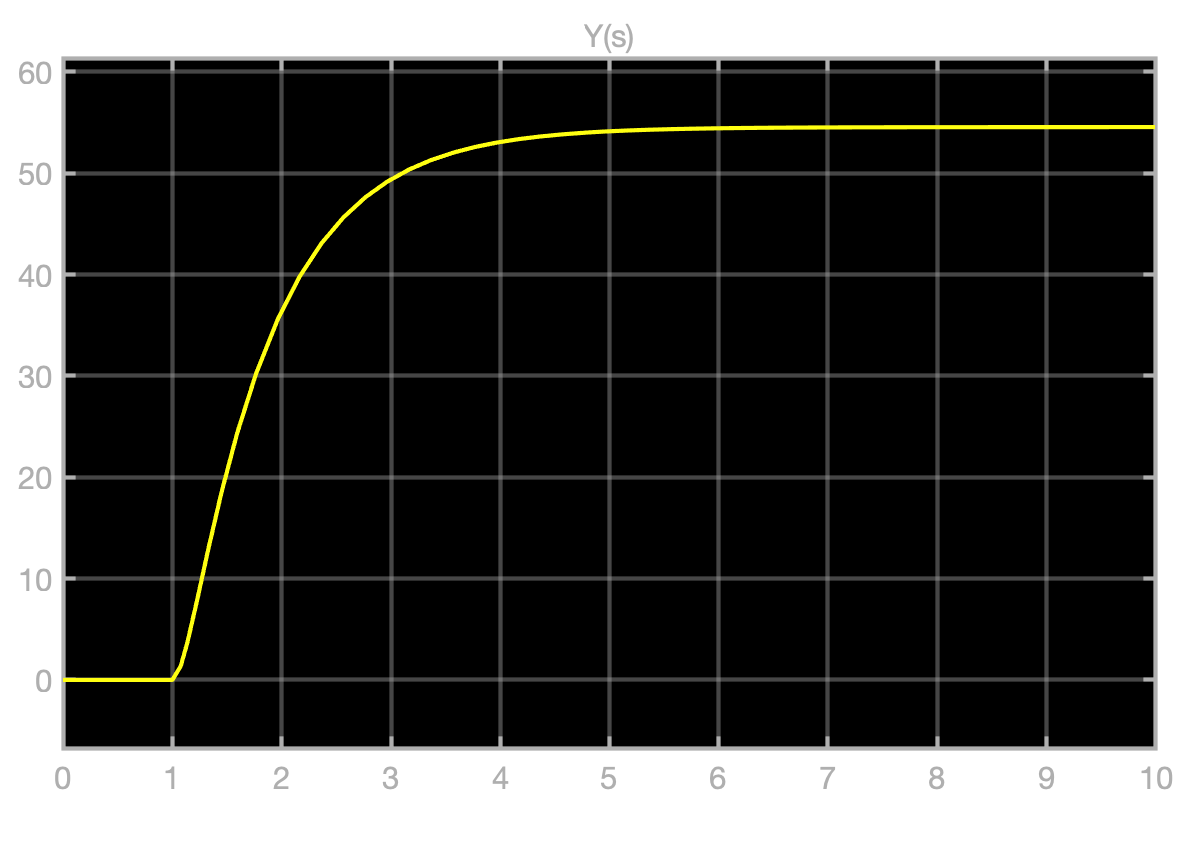
\includegraphics[width=\linewidth]{Bilder/UnderstandingPID_P_smallK.eps}
	\caption{Steady-state error with P-Control}
	\label{Fig_UnderstandingPID_P_ss_smallK}
\end{figure}
\begin{equation}\label{Eq_UnderstandingPID_P}
	\frac{Y(s)}{R(s)} = \frac{C(s)P(s)}{1 + C(s)P(s)} = \frac{b C(s)}{s^2 + as + b(1 + C(s))}
\end{equation}

\subsubsection{P Control}

Consider figure \ref{Fig_UnderstandingPID_P}, with P control, the control signal is given by $U(s) = K_P E(s)$ ($C(s) = K_P$), therefore, equation of the system \eqref{Eq_UnderstandingPID_P}, now becomes:
\begin{equation}
	\frac{Y(s)}{R(s)} = \frac{C(s)P(s)}{1 + C(s)P(s)} = \frac{b K_P}{s^2 + as + b(1 + C(s))}
\end{equation}
The terms in the above equation can be matched with the terms of the PT-2 canonical system in order to derive the system properties such as:
\begin{align}
	\omega_{n}^2 &= b(1 + K_P) \\
	2 \zeta \omega_{n} &= a
\end{align}
further $\omega_{n}$ and $\zeta$ are simplified as:
\begin{align}
	\omega_{n} &= \sqrt{b(1 + K_P)} \label{Eq_UnderstandingPID_P_wn} \\
	\zeta = \frac{a}{\omega_{n}} &= \frac{a}{2 \sqrt{b(1 + K_P)}} \label{Eq_UnderstandingPID_P_zeta}
\end{align}
It can be seen form equations \eqref{Eq_UnderstandingPID_P_wn} and \eqref{Eq_UnderstandingPID_P_zeta} that as $K_P$ the control gain is increased, $\omega_{n}$ increases and $\zeta$ decreased. Increasing $\omega_{n}$ and decreasing $\zeta$ says that as $K_P$ is increasing, the system is becoming more stiffer. Also noting that for this system the poles are shifted using only $K_P$ therefore, it is a 1 DOF system.

\textbf{Steady-state performance}

For a unit step reference:
\begin{equation}
	y_{ss} = \lim_{s\to 0} s Y(s) = \lim_{s\to 0} s \frac{C(s)P(s)}{1 + C(s)P(s)} = s \frac{b K_P}{s^2 + as + b(1 + K_P)} \frac{1}{s}
\end{equation}
the above equation simplifies to:
\begin{equation}\label{Eq_UnderstandingPID_P_ss}
	y_{ss} = \lim_{s\to 0} s Y(s) = \frac{K_P}{1 + K_P} \neq 1
\end{equation}
From equation \eqref{Eq_UnderstandingPID_P_ss}, it can be seen that the ratio is never equal to $1$ for a unit step reference. Therefore, mathematically it is impossible to track the system perfectly using P-Control. Further from equation \eqref{Eq_UnderstandingPID_P_ss}, it can be seen that as $K_P$ is made large enough, the denominator of equation \eqref{Eq_UnderstandingPID_P_ss} is dominated by $K_P$, thereby leading to a ratio which is very close to $1$. This is one of the ways to reduce the SS-error in the system as shwon in figure \ref{Fig_UnderstandingPID_P_ss_bigK}.
\begin{figure}[h!]
	\centering
	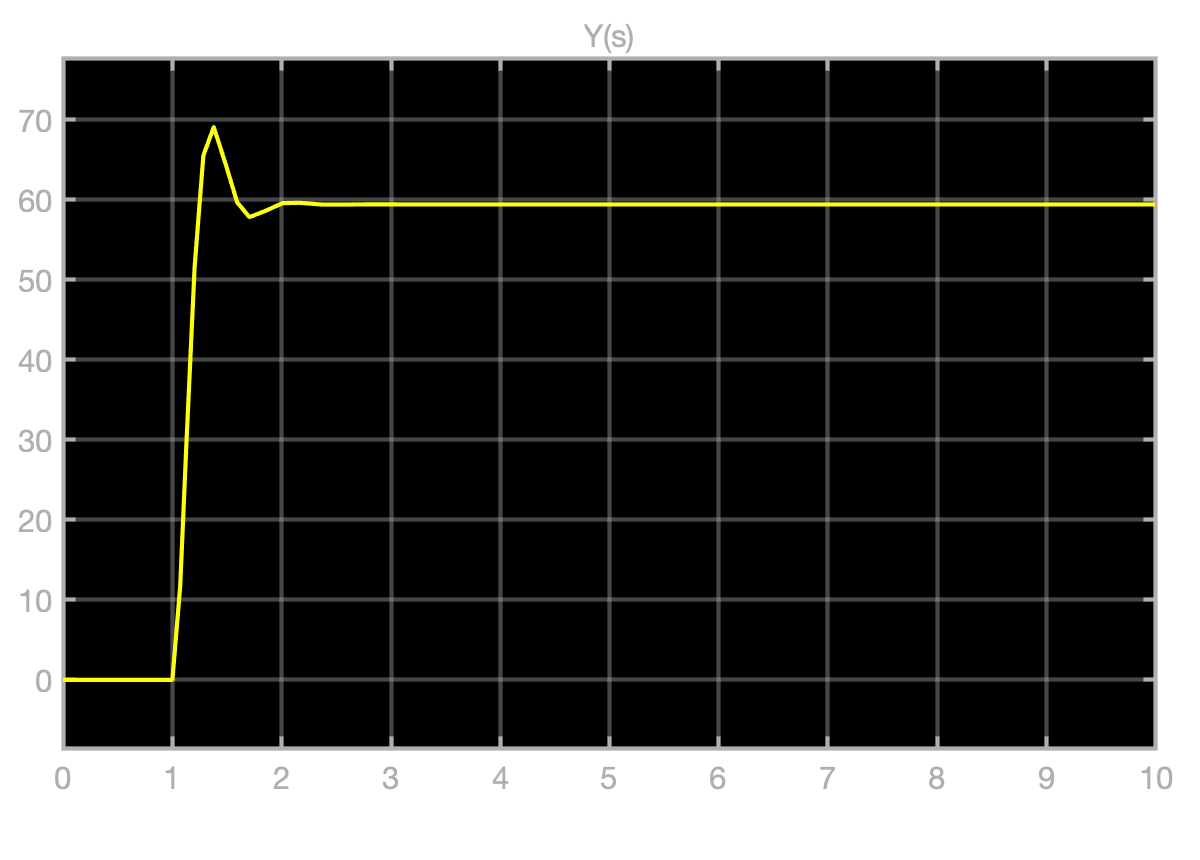
\includegraphics[width=\linewidth]{Bilder/UnderstandingPID_P_bigK.eps}
	\caption{Reduced Steady-state error with P-Control}
	\label{Fig_UnderstandingPID_P_ss_bigK}
\end{figure}
\newpage
However, it can also be seen in figure \ref{Fig_UnderstandingPID_P_ss_bigK}, increasing $K_P$ also increases overshoot and induces oscillations into the system which is evident from equations \eqref{Eq_UnderstandingPID_P_wn} and \eqref{Eq_UnderstandingPID_P_zeta} which indicated that higher $K_P$ would make the system stiffer and increase oscillations and overshoot (due to decreased damping).

\textbf{Tips: }Increasing the proportional gain $K_P$ tends to scale the error (control action) to the same level. As in a P control pushing harder will accelerate (system will react more quickly for higher $K_P$) the systems response more quickly it will also cause an overshoot. Increasing $K_P$ can reduce the ss-error but not eliminate it completely as proved using final value theorem on ss-error.

\subsubsection{D Control}

In a proportional only control, when a proportionally large control action needs to be given to the system due to rapidly increasing dynamics, the proportional control will have to wait until the value of the error itself increases. However, in a differential control the control looks at the slope of the error which in-turn reflects the rapid change in the dynamics. The slope will have started first in any curve before the curve reaches to its maximum value following that slope. Therefore, in a differential control as the control is given proportional to the slope, a massive control action can be given to the system even before it reaches the maximum change in state (value) as soon as the slope changes. This in essence is like predicting the future trends of the system dynamics and taking a necessary control action before hand (anticipating the future).

\textbf{Properties of derivative control}

Using figure \ref{Fig_NoiseDerivativeControl} and ignoring noise, the TF of the derivative control is expressed as $C(s) = K_D s$, therefore, the TF of the plant with noise as input can be written as:
\begin{equation} \label{Eq_UnderstandingPID_D_sys}
	\frac{Y(s)}{R(s)} = \frac{\frac{K_{D}s b}{s^2 + m s + b}}{1 + \frac{K_{D}s b}{s^2 + m s + b}} = \frac{K_{D}s b}{s^2 + (m + K_{D} b)s + b}
\end{equation}
Comparing equation \eqref{Eq_UnderstandingPID_D_sys} with PT-2 canonical system, the system properties can be defined as:
\begin{align}
	\omega_{n} &= \sqrt{b} \label{Eq_UnderstandingPID_D_wn_1} \\
	2 \zeta \omega_{n} = m + K_{D} b \implies \zeta &= \frac{m + K_{D} b}{2 \sqrt{b}} \label{Eq_UnderstandingPID_D_zeta_1}
\end{align}
As can be seen from equation \eqref{Eq_UnderstandingPID_D_wn_1}, the derivative control does not effect the natural frequency and in-turn the damped frequency of the system. The derivative control only effects the damping of the system as given in equation \eqref{Eq_UnderstandingPID_D_zeta_1}. It is a natural case of dynamic system that the derivative control can only effect the damping. As is the case with PT-2 systems, the damping is only present as a function of the first order derivative (velocity term) in the dynamic equation. The poles can be found using equations \eqref{Eq_UnderstandingPID_D_wn_1} and \eqref{Eq_UnderstandingPID_D_zeta_1}:
\begin{align}
	\sigma = \zeta \omega_{n} &= \frac{m + K_{D} b}{2 \sqrt{b}} \\
	\omega_{n}  &= \omega_{n} \sqrt{b}
\end{align}
From the above equations it can be seen that changing $K_D$ will effect only the real part of the pole as the imaginary part of the pole can be held constant by maintaining $K_D$ a constant. So changing $K_D$ will change the real part of the pole radially as the radius of the pole $\omega_{n}$ will always be a constant in this case. By increasing $K_D$, the angle $cos(\beta)$ will move more closely towards the real axis un-till the poles become repetitive in case of critical damping. As a derivative control increasing damping it cuts down the overshoots in the system as the property $M_p$ which determines the percentage overshoots is reduced exponentially due to the increase in $\zeta$. Further, the settling time $t_s = 4 / \sigma$ also reduces as $\sigma$ increases. Finally, the overshoot peak time $t_p = \pi / \omega_{n}$ will remain unaffected by $K_D$ as a derivative control does not change the location of pole radially.

The action of the derivative control reducing the overshoot of the system can be seen using the system as shown in figure \ref{Fig_UnderstandingPID_P}. It can be seen in figure \ref{Fig_UnderstandingPID_P_ss_bigK}, that a high $K_P$ increases the overshoot of the system which can be controlled by adding a derivative control such that $C(s) = K_P + K_D s$. Figure \ref{Fig_OvershootReduction_DerivativeControl} (produced with Matlab) shown the action of the derivative control reducing the overshoot in the system which acts a stabilizer as it damps the oscillations in the system.
\begin{figure}[h!]
	\centering
	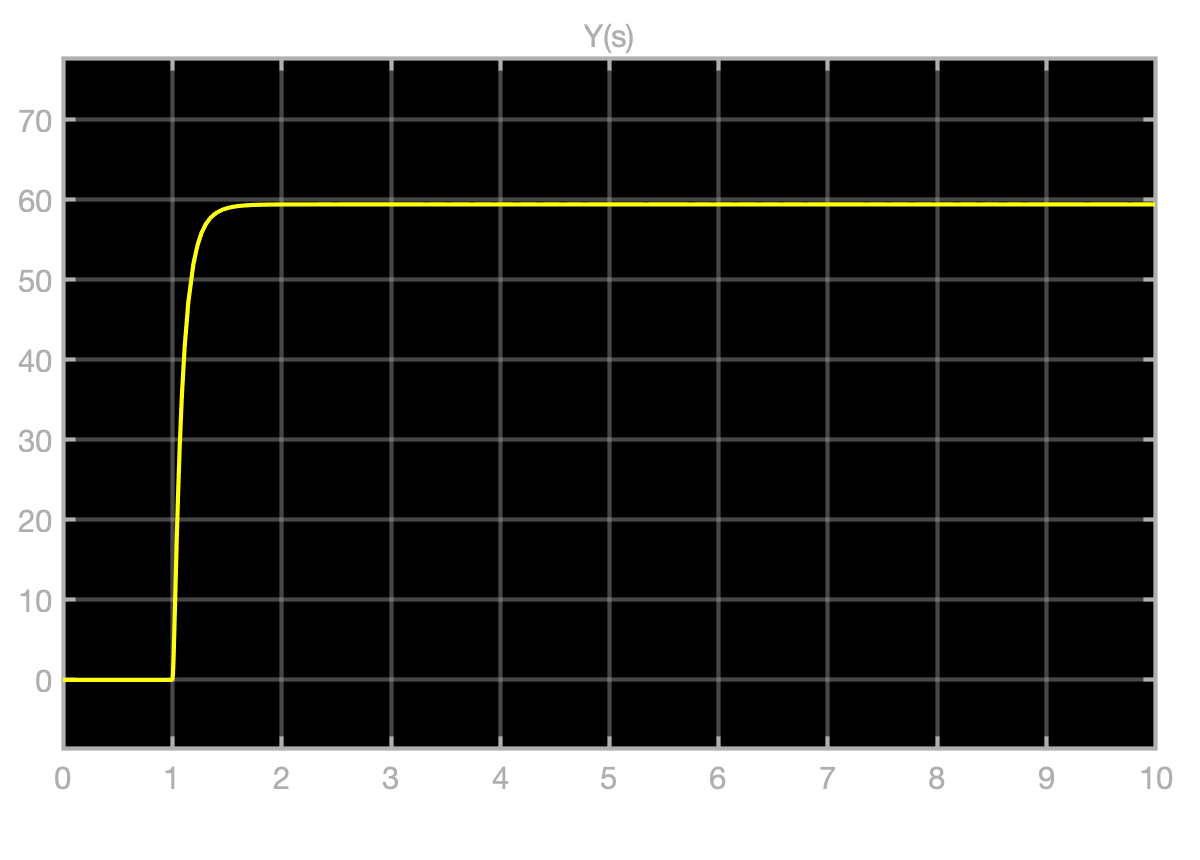
\includegraphics[width=\linewidth]{Bilder/UnderstandingPID_D_Overshoot.eps}
	\caption{Overshoot elimination using derivative control}
	\label{Fig_OvershootReduction_DerivativeControl}
\end{figure}
While designing the controller for an industry application, it is a common practice to first start with the proportional control and then use derivative control for reducing overshoot in the system or increasing damping or similar properties.

\textbf{Tip: }A P control will only increase if the error also increases, as a D contol will anticipate the trend of the error in advance by checking the slope, this anticipation will tend to add damping into the system, reducing the overshoot.

\textbf{Noise amplification in derivative control}

A D-control however cannot be used all by itself and is not generally used because of its nature to amplify the noise into the system. In order to study the effects of the noise in the system lets consider analytical solution of the system with noise as shown in figure \ref{Fig_NoiseDerivativeControl}.
\begin{figure}[h!]
	\centering
	\includegraphics[width=\linewidth]{Bilder/NoiseDerivativeControl.pdf}
	\caption{Performance of Derivative Control with noise}
	\label{Fig_NoiseDerivativeControl}
\end{figure}
writing the TF when noise $N(s)$ is input to the system:
\begin{equation}
	\frac{Y(s)}{N(s)} = \frac{\frac{- K_D s . b}{s^2 + ms + b}}{1 + \frac{K_D s . b}{s^2 + ms + b}}
\end{equation}
simplifying above equation:
\begin{equation}
	\frac{Y(s)}{N(s)} = \frac{- K_D s . b}{s^2 + (m + K_D b)s + b}
\end{equation}
the steady-state error of the output can be found using FVT and a unit step function as the noise signal $N(s)$:
\begin{equation} \label{Eq_UnderstandingPID_D_noise}
	ss_{y} = \lim_{s\to 0} s Y(s) = \lim_{s\to 0} s \frac{- K_D s . b}{s^2 + (m + K_D b)s + b} \frac{1}{s} = \infty
\end{equation}
Using Matlab the following simulation was produced with a derivative control \ref{Fig_Noiseamplification_DerivativeControl}. A derivative control always produces a steady-state error which increased to $\infty$ for any kind of input noise signal. A derivative control always has this effect of amplifying noise into the system. It is for this reason that in most of the industries a derivative control is avoided as far as possible.
\begin{figure}[h!]
	\centering
	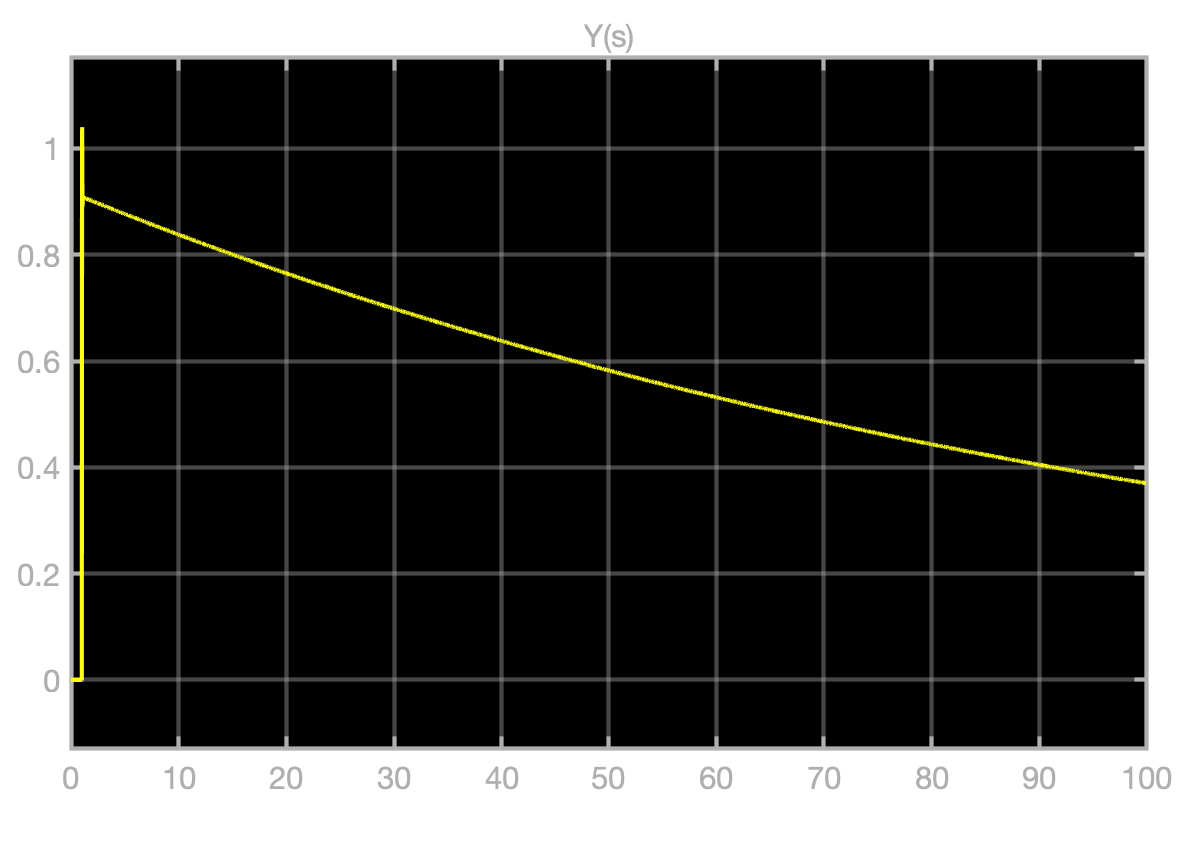
\includegraphics[width=\linewidth]{Bilder/NoiseAmplification_DerivativeControl.eps}
	\caption{Noise amplification of derivative control into the system}
	\label{Fig_Noiseamplification_DerivativeControl}
\end{figure}

\subsubsection{I Control}

An integral control adds new features to the system which are very helpful for the control in terms of achieving a perfect steady-state response. An integral control generally increases the order of the system, so a PT-1 system with an integral control will become a PT-2 system and so on. By doing so it is intuitively easier to understand that the higher order system are generally more oscillating and have longer settling times compared to their lower counter-parts. That what the integral control does to the system, it generally increases the oscillations in the system and makes the system slower. It is generally difficult to analyses systems with integral control, an attempt is made to come up with a most simplest example. Consider a PT-1 system of the canonical form:
\begin{equation} \label{Eq_UnderstandingPID_I_PT1}
	P(s) = \frac{1}{\tau s + 1}
\end{equation}
with an integral control $C(s) = K_I / s$, the forward TF for the system can be expressed as:
\begin{equation}
	G(s)_{f} = \frac{K_I}{s(\tau s + 1)} = \frac{K_I}{s^2 \tau + s}
\end{equation}
the TF of the system (for a negative feedback) can be expressed as:
\begin{equation}
	G(s) = \frac{Y(s)}{R(s)} = \frac{forward}{1 + loop} = \frac{\frac{K_I}{s^2 \tau + s}}{1 + \frac{K_I}{s^2 \tau + s}}
\end{equation}
simplifying the above equation:
\begin{equation} \label{Eq_UnderstandingPID_I_PT2}
	G(s) = \frac{K_I}{\tau s^2 + s + K_I} = \frac{K_I}{ s^2 + s / \tau + K_I / \tau}
\end{equation}
It can be seen just by analyzing equations \eqref{Eq_UnderstandingPID_I_PT1} which was the previous order of the system without integral control and the current system equation \eqref{Eq_UnderstandingPID_I_PT2} which is now a PT-2 system. Generally a PT-1 system has only one pole at $s = -1 / \tau$ whereas a PT-2 system has two poles of complex conjugate in nature which can be found in case of equation \eqref{Eq_UnderstandingPID_I_PT2} by comparing with the canonical PT-2 system:
\begin{align}
	\omega_{n} &= \sqrt{\frac{K_I}{\tau}} \\
	2 \zeta \omega_{n} = \sigma \implies 2 \zeta \omega_{n} &= 1 / \tau
\end{align}
there are two observation that can be made at this point, the real part of the pole $\sigma = 1 / \tau$ is a constant and will remain fixed in the complex plane. The Im part can be placed in the complex plane by changing $K_I$ which will increase the vertical placement of the pole along the Im axis. This increases the angle $\cos{\beta}$ which will increase the oscillations in the system. Therefore, it can be proved with this simple example that an integral control will induce oscillations into the system firstly by increasing the poles in the system and also by placing the poles away by increasing angle $cos{\beta}$.

The effect of increasing settling time increase by the integral control is complicated at this time. But according to the error build-up concept explained in \cite[t.1:01:00]{RickHill_14}, if the error in the system changes its sign, the control action proportional to it does not change its sign. This would lead to undoing the control action in the next cycle when the error changes the direction again. Therefore, an integral control makes the system slower to settle down compared to proportional and derivative controls.

\textbf{Tip: }The I control reduces the ss-error by increasing the control action which results due to the persistent built-up of the ss-error. This build-up gets summed up by the integrator and so will be the control action as a result of it. The I control makes the system slow because if the error signal changes the sign then due to that addition of the overall built-up error, the change in error sign will partly cancel out the previously built-up error in summation. Therefore, it will take some time for the I control to "unwind" from changing signs in error signals.

\subsection{PD Control}

A PD control for a second order canonical system can be used to determine the control system behavior. The PD control is expressed as $C(s) = K_P + K_D s$, for the system shown in figure \ref{Fig_NoiseDerivativeControl} ignoring noise, the TF of the system with PD control can be expressed as:
\begin{equation} \label{Eq_UnderstandingPID_PD_sys}
	G(s) = \frac{Y(s)}{R(s)} = \frac{b(K_P + K_D s)}{s^2 + (m+b K_D)s + b(1 + K_P)}
\end{equation}
From equation \ref{Eq_UnderstandingPID_PD_sys}, it can be seen that the derivative control term again works in conjunction with the damping term of the PT-2 canonical system. Therefore, in summary to applying individual proportional and integral controls is that $K_P$ will change the $\omega_{n}$ of the system independently \{1 DOF\} and $K_D$ will only change the damping $\zeta$ of the system independently \{1 DOF\}. Which leads to the fact that with a PD control now it is possible to combine the poles of the system independently for either increasing stiffness $\omega_{n}$ or increase the damping $\zeta$ independently \{2 DOF\} (can place the poles anywhere). Also with the PD control the steady-state error of the system remains the same as that of the ss error when using only P control as can be seen from equation \eqref{Eq_UnderstandingPID_PD_sys}. That also means that the steady-state error amplification due to noise seen by using only derivative control (equation \eqref{Eq_UnderstandingPID_D_noise}) will be eliminated and replaced with equation \eqref{Eq_UnderstandingPID_P_ss}.

\subsubsection{PI Control} \label{Sec_UnderstandingPID_PI}

An integral control acts on the basis of the time history of the accumulated errors and therefore gets larger as errors get accumulated over time. An advantage of using a PI control in combination is that the integral action will lead the system to a perfect tracking of the steady-state response. Consider a PI control for the system shown in figure \ref{Fig_UnderstandingPID_P} with control action $$C(s) = K_P + K_I / s$$, the TF of such system can be expressed as:
\begin{equation}
	\frac{Y(s)}{R(s)} = \frac{b\left(K_P + K_I / s \right)}{s^2 + as + b\left(1 + K_P + K_I / s\right)} = \frac{b(K_P s + K_I)}{s^3 + as^2 + b(1 + K_P)s + bK_I}
\end{equation}
the steady-state performance of the system can be found using FVT:
\begin{equation}
	y_{ss} = \lim_{s\to 0} s Y(s) = \lim_{s\to 0} s \frac{b(K_P s + K_I)}{s^3 + as^2 + b(1 + K_P)s + bK_I} \frac{1}{s} = \frac{b K_I}{b K_I} = 1
\end{equation}
therefore, by using an integral control in conjunction with proportional control makes the ss-error of the system zero. This is true even if $K_I$ is small (however, a bigger $K_I$ will be much faster).

\subsubsection{Summarizing PID control actions}

The summary of each term can be best visualized using the following table:
\begin{table}[h!]
	\centering
	\begin{tabular}{p{2.5cm} | p{4cm} | p{3cm} | p{3cm}}
		\toprule
		Control & Action & Pros & Cons \\
		\cmidrule{1-4}
		Proportional & Proportional action w.r.t error & Fast reponse & Increases Overshoot \\
		Differential & Anticipates error using slope & Adds damping (reduces overshoot and $t_s$) & Amplifies noise into the system \\
		Integral & Control builds up as erro builds up & Reduce steady-state error & Induces oscillations and makes the system slow to settle down \\
		\bottomrule
	\end{tabular}
\end{table}

\textbf{Note:} This intuition is developed using only PT-2 canonical system, the results may vary for other systems. The most important thing is to check for the location od poles and zeros in the overall system after adding the controls. However, for higher order non-canonical system, model order reduction techniques could be used to reduce the system to PT-1 or PT-2. Only trail and errro method is used to determine the effect of PID control action on non-canonical systems.

\section{System Type - Steady-state error}

As can be seen from section \ref{Sec_UnderstandingPID_PI}, using an integral action in the cases of the canonical system type always leads to a perfect steady-state tracking, essentially bringing the steady-state error of the system to zero. This integral action does not need be only in the controller level but integral actions are sometimes inherent in the plant itself. Basically, it is the pole placement of the integral action. The integral control always places the poles at the origin as can be seen with the transfer function of the an I-Control $C(s) = K_I / s$, such a control with a PT-1 plant, the OL TF of the system:
\begin{equation}
	G(s) = \frac{K_I}{s(\tau s + 1)}
\end{equation}
it can be seen that this system has two poles, one at $s_1 = -1/\tau$ and other at $s = 0$ due to the pole made by the integral control. Therefore, an integral control will always make a new pole at origin when used in any kind of system. Using the above result certain system types can be formalized among control systems using the following definition.

\textbf{System Type}: The number of poles at the origin in the forward path of a \textbf{\textit{unity feedback}} control system is called the system's type.

With poles either in the controller or in the plant itself. The following system types can now be defined:

\textbf{Type 0}: System with no poles at the origin
\begin{equation}
	G(s) = \frac{s + 1}{s + 4}
\end{equation}
\textbf{Type 1}: System with one pole at the origin
\begin{equation}
G(s) = \frac{s + 1}{s(s + 4)}
\end{equation}
\textbf{Type 2}: System with two poles at the origin
\begin{equation}
G(s) = \frac{s + 1}{s^2(s + 4)}
\end{equation}
\textbf{Type $n$}: System with one pole at the origin
\begin{equation}
G(s) = \frac{s + 1}{s^{n}(s + 4)}
\end{equation}
A system type which includes the reference in its TF can track the signal perfectly. For ex: Type 1 will track input with unit step and Type 2 will track input with unit ramp perfectly and so on. The following table provides some conclusions using various system types with various input signal types.
\begin{table}[h!]
	\centering
	\begin{tabular}{p{2.5cm} | p{3cm} | p{3cm} | p{3cm}}
		\toprule
				& \textbf{Step input} $r(t) = 1$ $R(s) = 1/s$ & \textbf{Ramp input} $r(t) = t$ $R(s) = 1 / s^2$ & \textbf{Acceleration input} $r(t) = \frac{1}{2}t^2$ $R(s) = 1 / s^3$ \\
				\cmidrule{1-4} \\
		\textit{Type 0} & nonzero & $\infty$ & $\infty$ \\
		\textit{Type 1} & 0 & nonzero & $\infty$ \\
		\textit{Type 2} & 0 & 0 & nonzero \\
		\bottomrule
	\end{tabular}
	\caption{Table summarizing standard system types with standard input types}
\end{table}